In this section we describe the experimental results we have obtained using Cerebro and the associated tools. We conduct
tests using five sample applications. 

\begin{description}
\item[StudentInfo] A JAXRS application for managing students of a class. Provides APIs for
adding/removing students, and listing the student information.
\item[ServerHealth] An application that monitors a given web URL for server uptime. Provides an
API for obtaining the uptime statistics computed by the application.
\item[SocialMapper] A simple social networking application. Provides APIs for adding users,
comments and other resources.
\item[StockTrader] A stock trading application. Provides APIs for adding users, registering
companies, buying and selling stocks among users.
\item[Rooms] A hotel booking application. Provides APIs for registering hotels and looking up
available rooms.
\end{description}

We instrument each of the above applications to measure the time taken by their web APIs to execute the
enclosed code. This is done by adding some extra Java code to each of the web APIs exposed by the sample applications.
We ensure that the instrumentation does not alter the original web API code in anyway (i.e. the original algorithms, control flow
and data flow are not impacted by the instrumentation). Then for each application we also
implement a mechanism to output the measured execution times, so an external client can query and collect the execution
times of the web APIs.

We carry out each of our tests in two separate environments -- Google App Engine public cloud, and
the AppScale private cloud. The AppScale private cloud used for testing was powered by four m3.2xlarge virtual machines 
running on a private Eucalyptus cluster.

In the first set of experiments, we benchmark each application for a period of 15 to 20 hours.
During this time, we run an HTTP client on a separate machine that invokes the instrumented web APIs once every minute, 
and collects the server-side execution times (as measured by the instrumentation code).
At the same time, we also run Watchtower in the same target cloud environment as the test application to
benchmark the individual cloud SDK operations. Our five sample applications extensively use the datastore cloud SDK 
operations of Google App Engine. The Rooms application also makes use of the memcache cloud SDK operations. Hence,
we configure Watchtower to periodically benchmark the cloud SDK operations related to datastore and memcache. 
At the end of a benchmarking run, we have two sets of data at hand:

\begin{itemize}
\item Web API execution times collected by the benchmarking HTTP client
\item Cloud SDK benchmarking data gathered by Watchtower
\end{itemize}

We now run Cerebro to make predictions regarding the web API execution time using the cloud SDK benchmarking data
collected by Watchtower. We configure Cerebro to predict an upper bound for the 95th percentile of the web API
execution time, with an upper confidence of 0.01. Cerebro generates a sequence of execution time predictions -- one 
per minute. Then we compare these predictions against the actual web API execution times collected during the same
time period. More specifically, we approximately align the sequence of predictions with the time series of actual execution
times, and check whether each prediction is correct (i.e. prediction is equal to or higher than the
corresponding actual value). We then use the results to compute a running tally of the percentage accuracy of Cerebro
predictions over time.

\begin{figure}
\centering
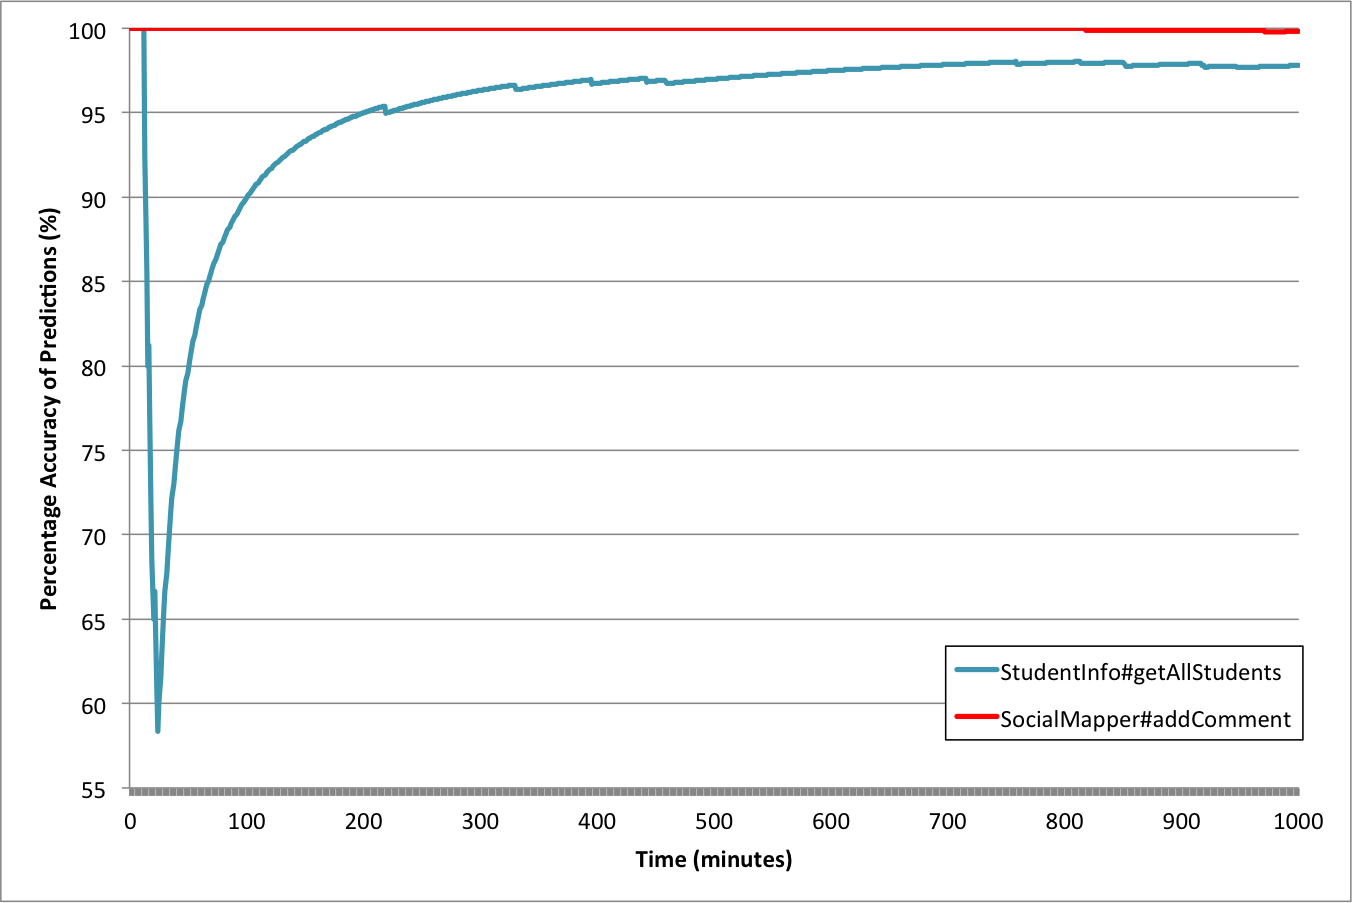
\includegraphics[scale=0.35]{gae_accuracy}
\caption{Percentage accuracy of predictions made on Google App Engine.}
\label{fig:gae_accuracy}
\end{figure}

Figure~\ref{fig:gae_accuracy} shows the percentage accuracy of the Cerebro predictions made in the Google App Engine 
public cloud environment. Each of the curves correspond to an single web API operation in one of the sample applications. 
The curves are labeled in the form of \textit{ApplicationName\#OperationName}. To maintain clarity in the figures we do not 
illustrate the results for all web API operations in the sample applications. Instead we present the results for a selected set of 
web API operations covering all five sample applications. We note that other web API operations we tested also produce
very similar results.

As expected QBETS takes some time to learn
from the time series data captured by Watchtower. This is when we see large fluctuations in the percentage accuracy. But
once QBETS has converged it consistently produces highly accurate predictions regarding the 95th percentile of the web API
response time. In the worst case QBETS takes up to 200 minutes to converge. This is the case with the
StudentInfo\#getAllStudents operation. After 275 minutes, we see highly accurate predictions being made on all web API
operations considered in the tests. After this point, we consistently see percentage accuracy values higher than 96\%. Note that
we had configured Cerebro to predict the 95th percentile of the web API executions time. Therefore as long as Cerebro produces
results with a percentage accuracy close to or higher than 95\%, we can consider the predictions as correct and reliable.

Figure 2 shows the same results calculated by running the sample applications and the Watchtower in the AppScale private cloud
environment.